\documentclass[a4paper,14pt]{extreport} % формат документа

\usepackage{amsmath}
\usepackage{cmap} % поиск в ПДФ
\usepackage[T2A]{fontenc} % кодировка
\usepackage[utf8]{inputenc} % кодировка исходного текста
\usepackage[english,russian]{babel} % локализация и переносы
\usepackage[left = 2cm, right = 1cm, top = 2cm, bottom = 2 cm]{geometry} % поля
\usepackage{listings}
\usepackage{graphicx} % для вставки рисунков
\usepackage{amsmath}
\usepackage{float}
\usepackage{multirow}
\graphicspath{{img/}}
\DeclareGraphicsExtensions{.pdf,.png,.jpg}
\newcommand{\anonsection}[1]{\section*{#1}\addcontentsline{toc}{section}{#1}}

\lstset{ %
	language=Lisp,                % Язык программирования 
	numbers=left,                   % С какой стороны нумеровать          
	frame=single,                    % Добавить рамку
}

\begin{document}
\begin{titlepage}

    \begin{table}[H]
        \centering
        \footnotesize
        \begin{tabular}{cc}
            \multirow{8}{*}{
\includegraphics[scale=0.35]{bmstu.jpg}}
            & \\
            & \\
            & \textbf{Министерство науки и высшего образования Российской Федерации} \\
            & \textbf{Федеральное государственное бюджетное образовательное учреждение} \\
            & \textbf{высшего образования} \\
            & \textbf{<<Московский государственный технический} \\
            & \textbf{университет имени Н.Э. Баумана>>} \\
            & \textbf{(МГТУ им. Н.Э. Баумана)} \\
        \end{tabular}
    \end{table}

    \vspace{-2.5cm}

    \begin{flushleft}
        \rule[-1cm]{\textwidth}{3pt}
        \rule{\textwidth}{1pt}
    \end{flushleft}

    \begin{flushleft}
        \small
        ФАКУЛЬТЕТ
        \underline{<<Информатика и системы управления>>\ \ \ \ \ \ \ 
        \ \ \ \ \ \ \ \ \ \ \ \ \ \ \ \ \ \ \ \ \ \ \ \ \ \ \ \ \ \ \ 
    \ \ \ \ \ \ \ \ \ \ \ \ \ \ \ } \\
        КАФЕДРА
        \underline{<<Программное обеспечение ЭВМ и
        информационные технологии>>
        \ \ \ \ \ \ \ \ \ \ \ \ \ \ \ \ \ \ \ \ }
    \end{flushleft}

    \vspace{2cm}

    \begin{center}
        \textbf{Лабораторная работа № 6} \\
        \vspace{0.5cm}
    \end{center}

    \vspace{4cm}

    \begin{flushleft}
        \begin{tabular}{ll}
            \textbf{Дисциплина} & Экономика программной инженерии.  \\
            \textbf{Тема} & Предварительная оценка параметров программного проекта \\
            \\
            \textbf{Студенты} & Сиденко А.Г.\\
            \textbf{Группа} & ИУ7-83Б \\
            \textbf{Оценка (баллы)} & \\
            \textbf{Преподаватель} & Барышникова М.Ю., Силантьева А.В.   \\
        \end{tabular}
    \end{flushleft}

    \vspace{4cm}

   \begin{center}
        Москва, 2021 г.
    \end{center}

\end{titlepage}

\begin{enumerate}

\item \textbf{Постановка задачи}

Исследовать влияние атрибутов программного продукта (RELY, DATA и CPLX) на трудоемкость (РМ) и время разработки проекта (ТМ) для базового уровня модели COCOMO и разных типов проектов (обычного, встроенного, промежуточного). Для этого получить значения PM и ТМ по всем типам проектов для одного и того же значения размера программного кода SIZE при отсутствии ограничений на время выполнения, выбрав номинальное значение параметра TIME. Какой из трех указанных драйверов затрат оказывает большее влияние на сроки реализации проекта и объем работ? Проанализировать, как изменятся значения PM и ТМ при наличии более жестких ограничений на время выполнения.

\item \textbf{Методика COCOMO}
\begin{itemize}
\item Атрибуты прогарммного продукта
\begin{itemize}
\item Требуемая надежность
\item Размер БД 
\item Сложность продукта
\end{itemize}
\item Атрибуты компьютера
\begin{itemize}
\item Ограничения времени выполнения
\item Ограничения объема основной памяти
\item Изменчивость виртуальной машины 
\item Время реакции компьютера
\end{itemize}
\item Атрибуты персонала
\begin{itemize}
\item Способности аналитика
\item Знание приложений
\item Способности программиста
\item Знание виртуальной машины
\item Знание языка программирования
\end{itemize}
\item Атрибуты проекта
\begin{itemize}
\item Использование современных методов
\item Использование программных инструментов
\item Требуемые сроки разработки
\end{itemize}
\end{itemize}

Каждому из этих 15 факторов ставится в соответствие рейтинг по шести бальной шкале, начиная от «очень низкий» и до «очень высокого» (по значению или важности фактора). Далее значения рейтинга заменяются множителями трудоемкости из таблицы.

Далее используя следующие формулы мы можем получить значения трудозатрат и времени разработки.

Трудозатраты= $C_1\cdot EAF \cdot \text{Размер}^{p_1}$

Время = $C_2 \cdot \text{Трудозатраты}^{p_2}$

Изначально возьмем все значения номинальными и по заданию варианта будем менять RELY, DATA и CPLX.

\begin{figure}[H]
  \centering
  \caption{Атрибуты. }
  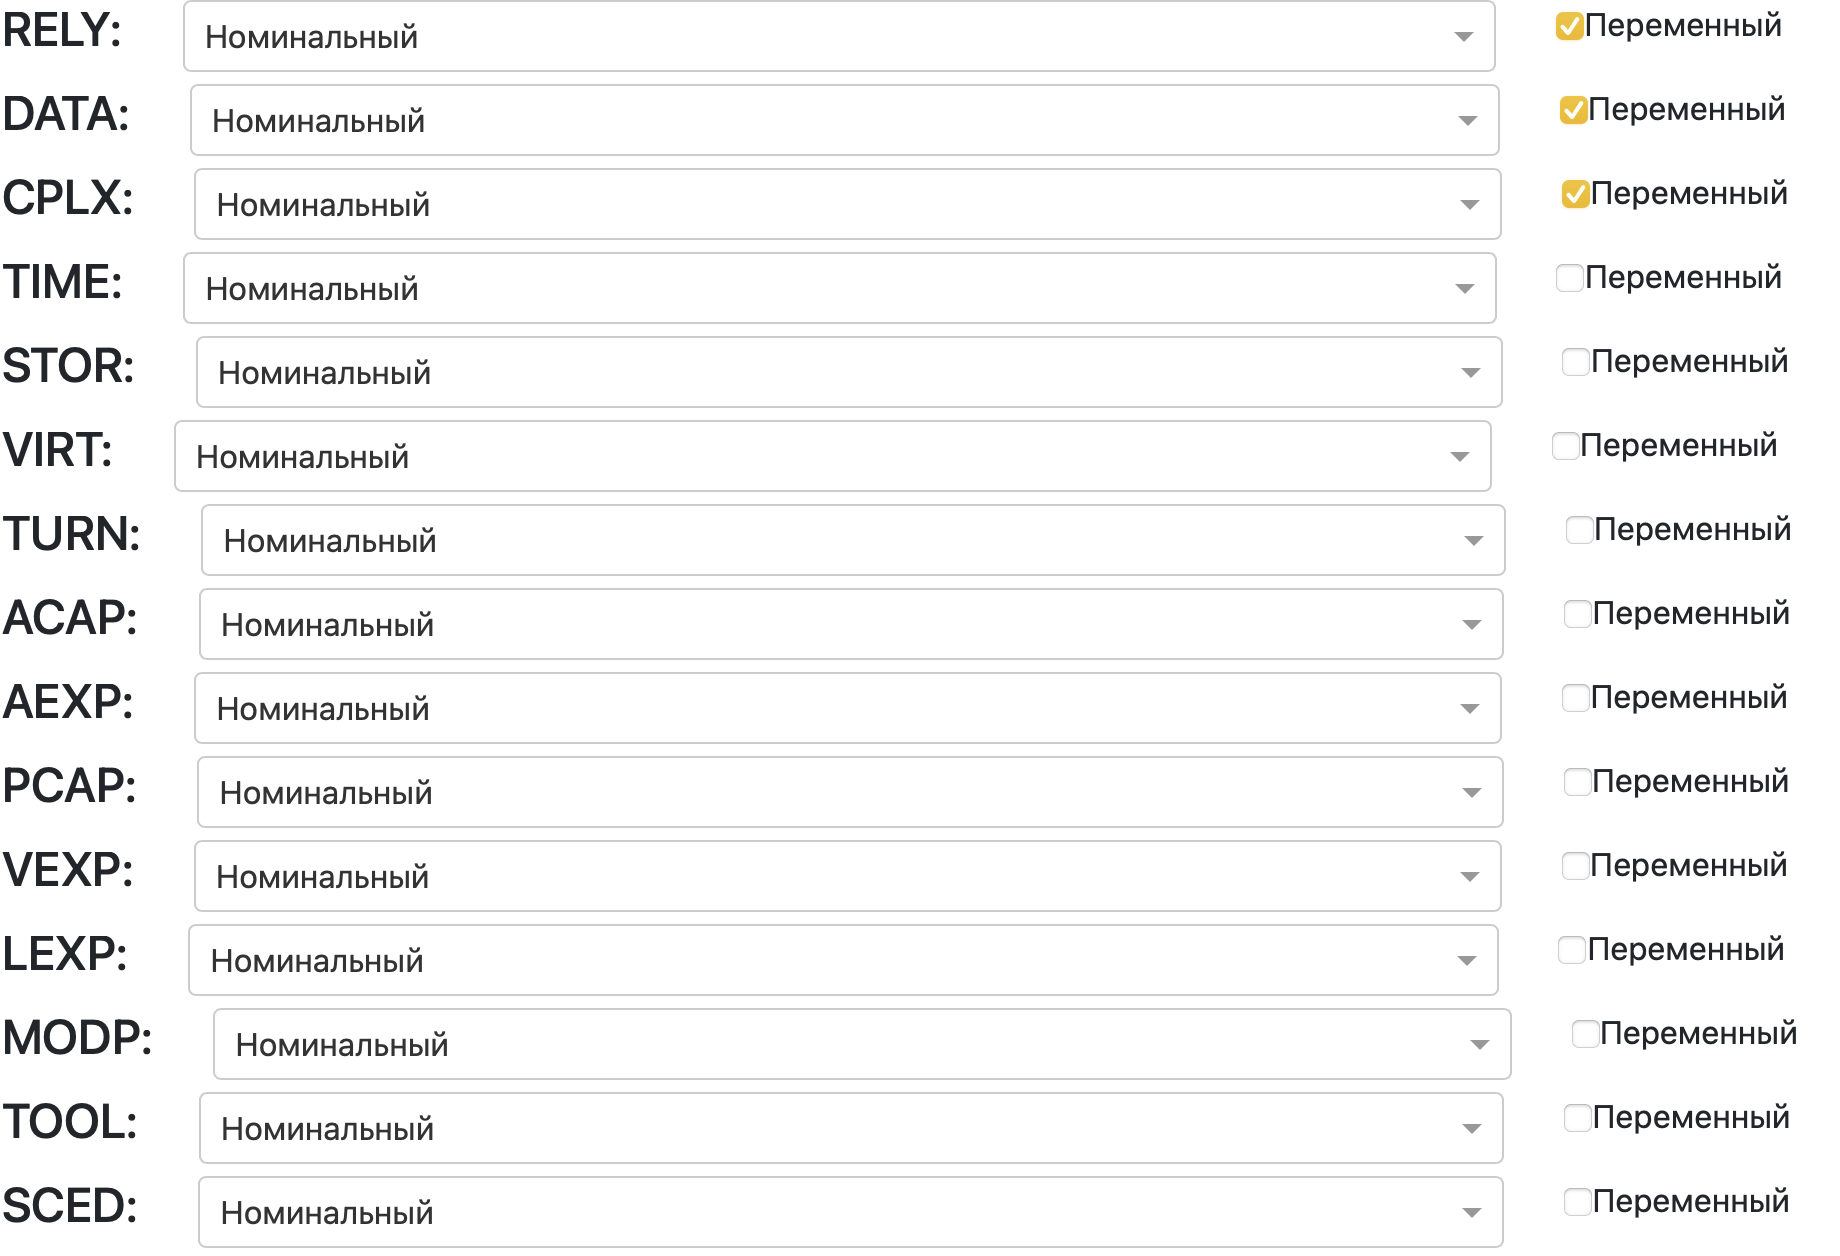
\includegraphics[scale=0.5]{table}
\end{figure}

\begin{figure}[H]
  \centering
  \caption{Изменение атрибутов в обычном типе проекта. }
  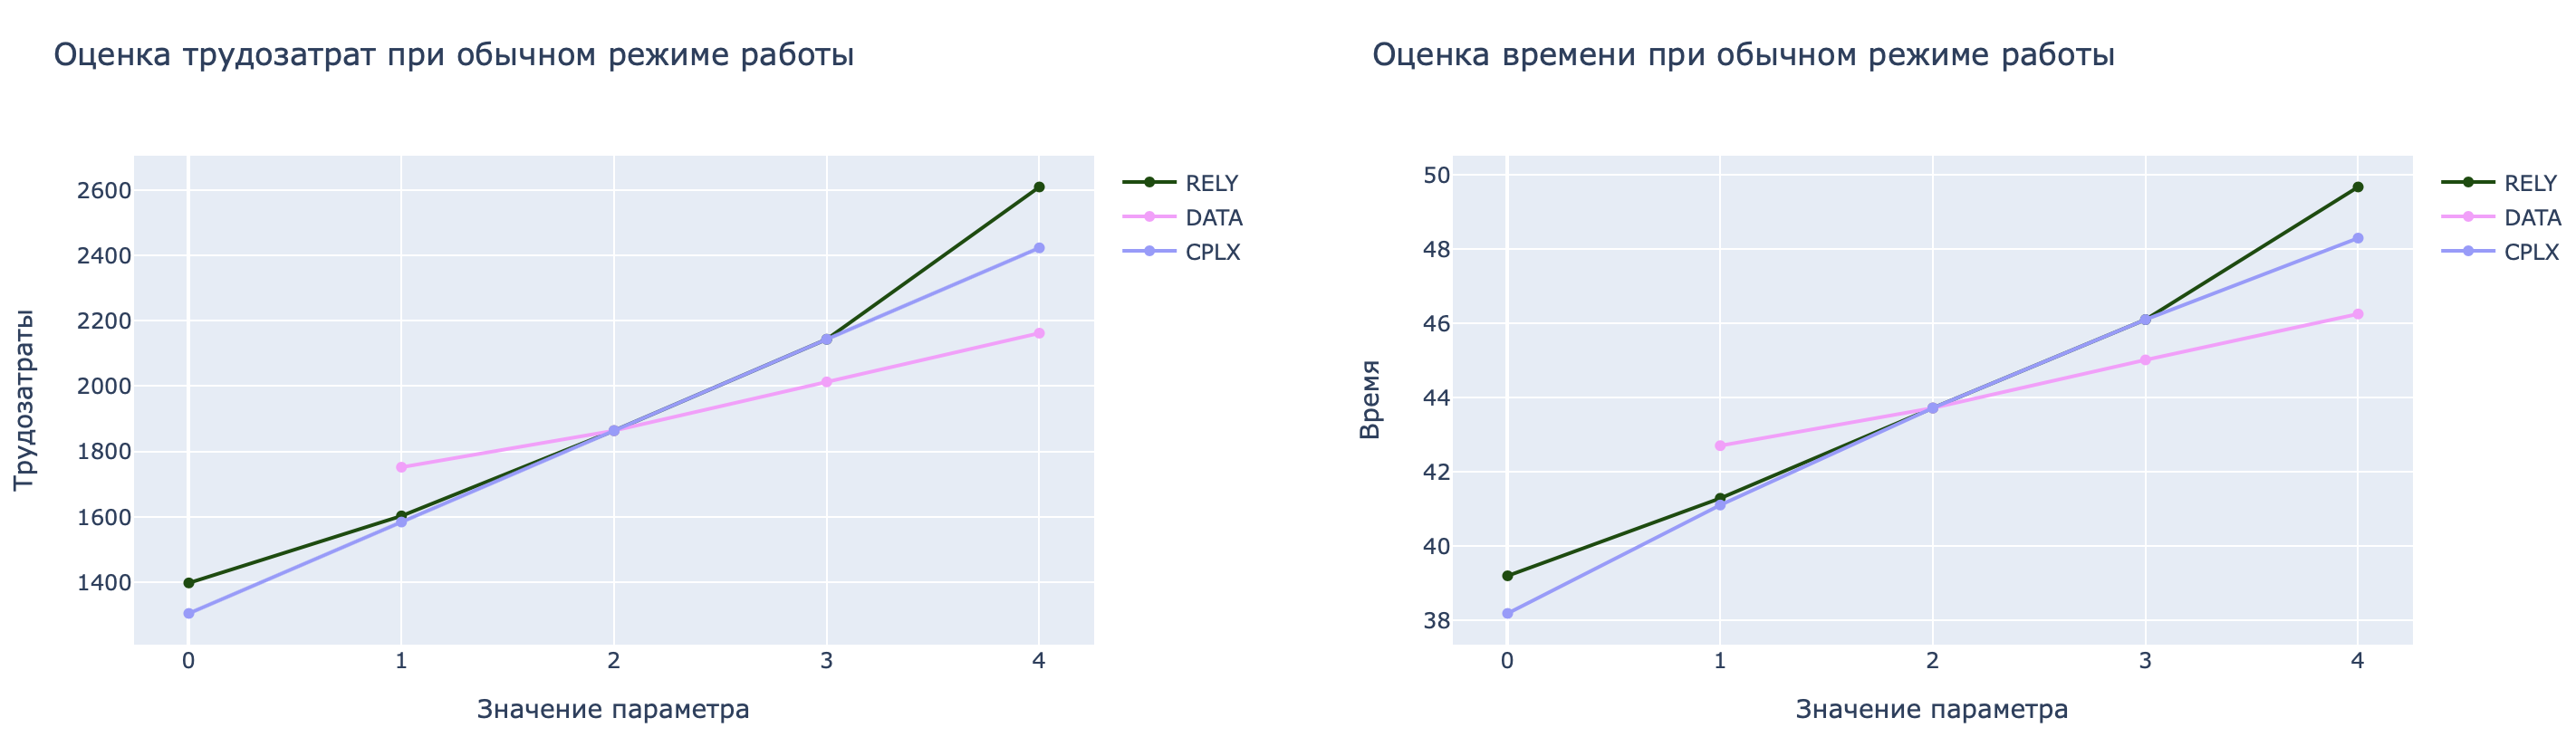
\includegraphics[scale=0.4]{norma}
\end{figure}

\begin{figure}[H]
  \centering
  \caption{Изменение атрибутов в промежуточном типе проекта. }
  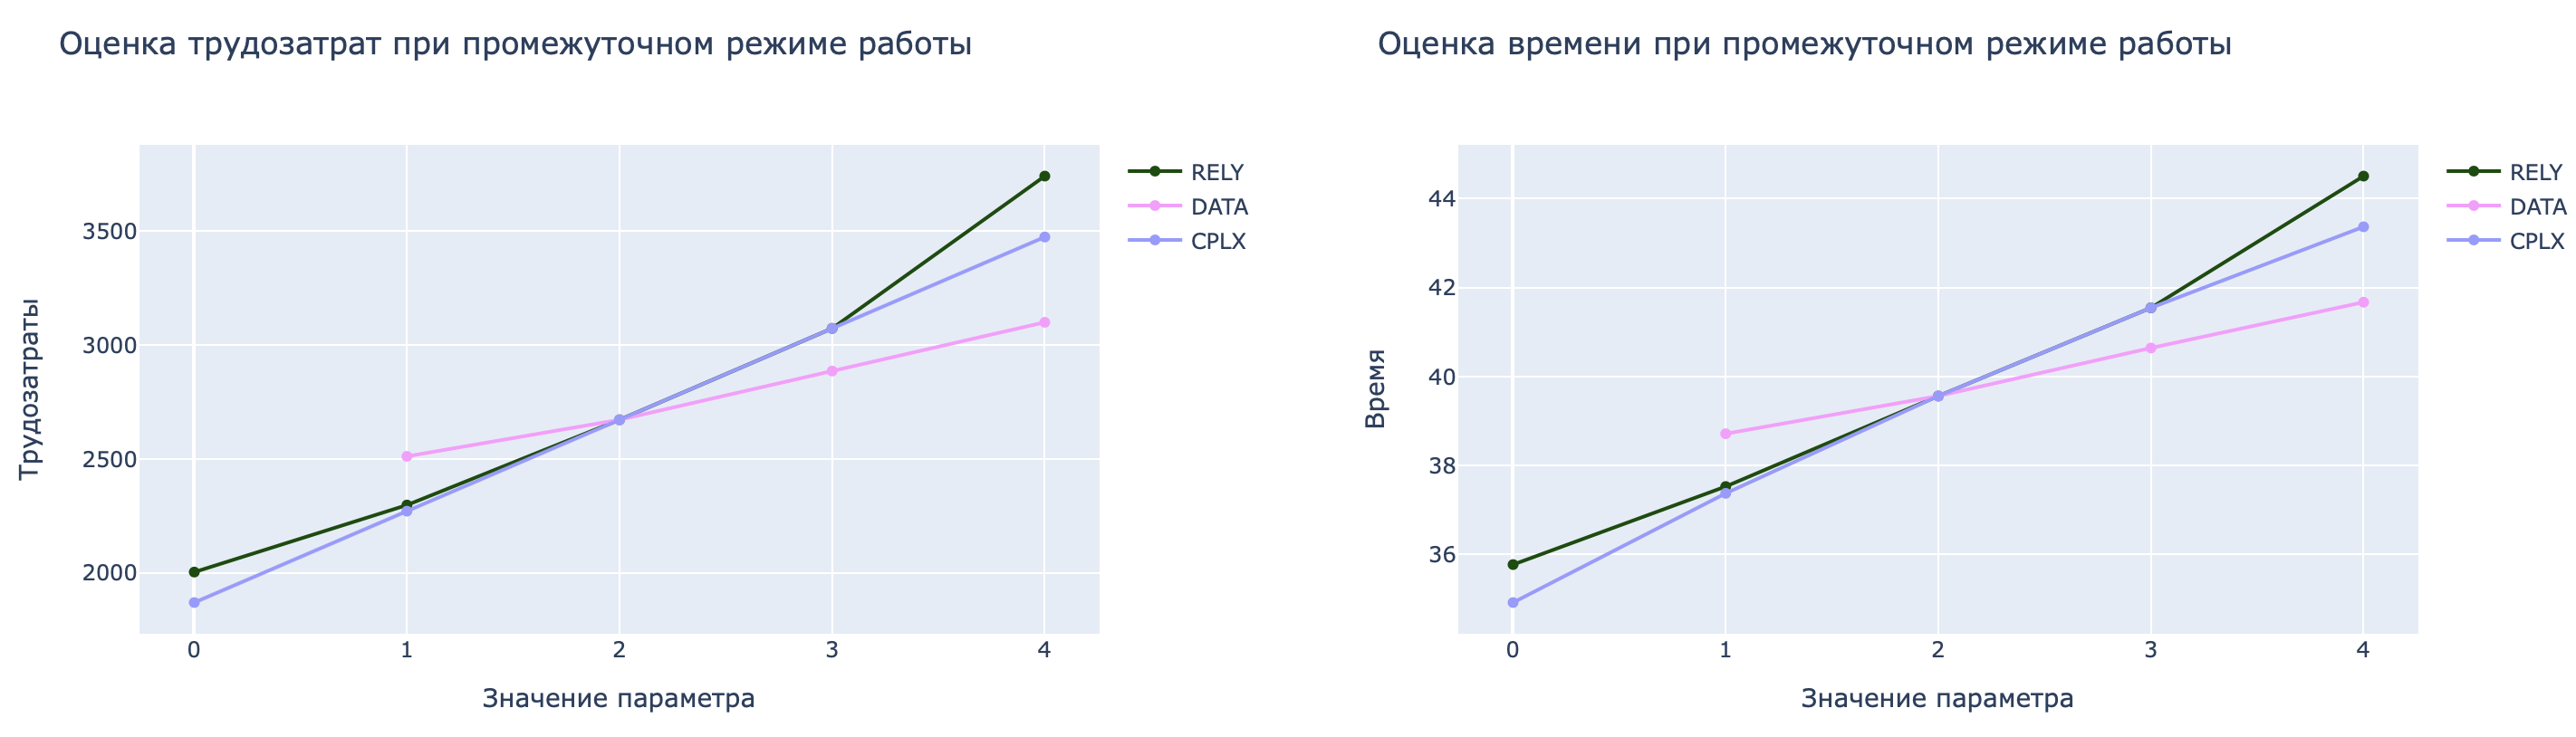
\includegraphics[scale=0.4]{interm}
\end{figure}

\begin{figure}[H]
  \centering
  \caption{Изменение атрибутов во встроенном типе проекта. }
  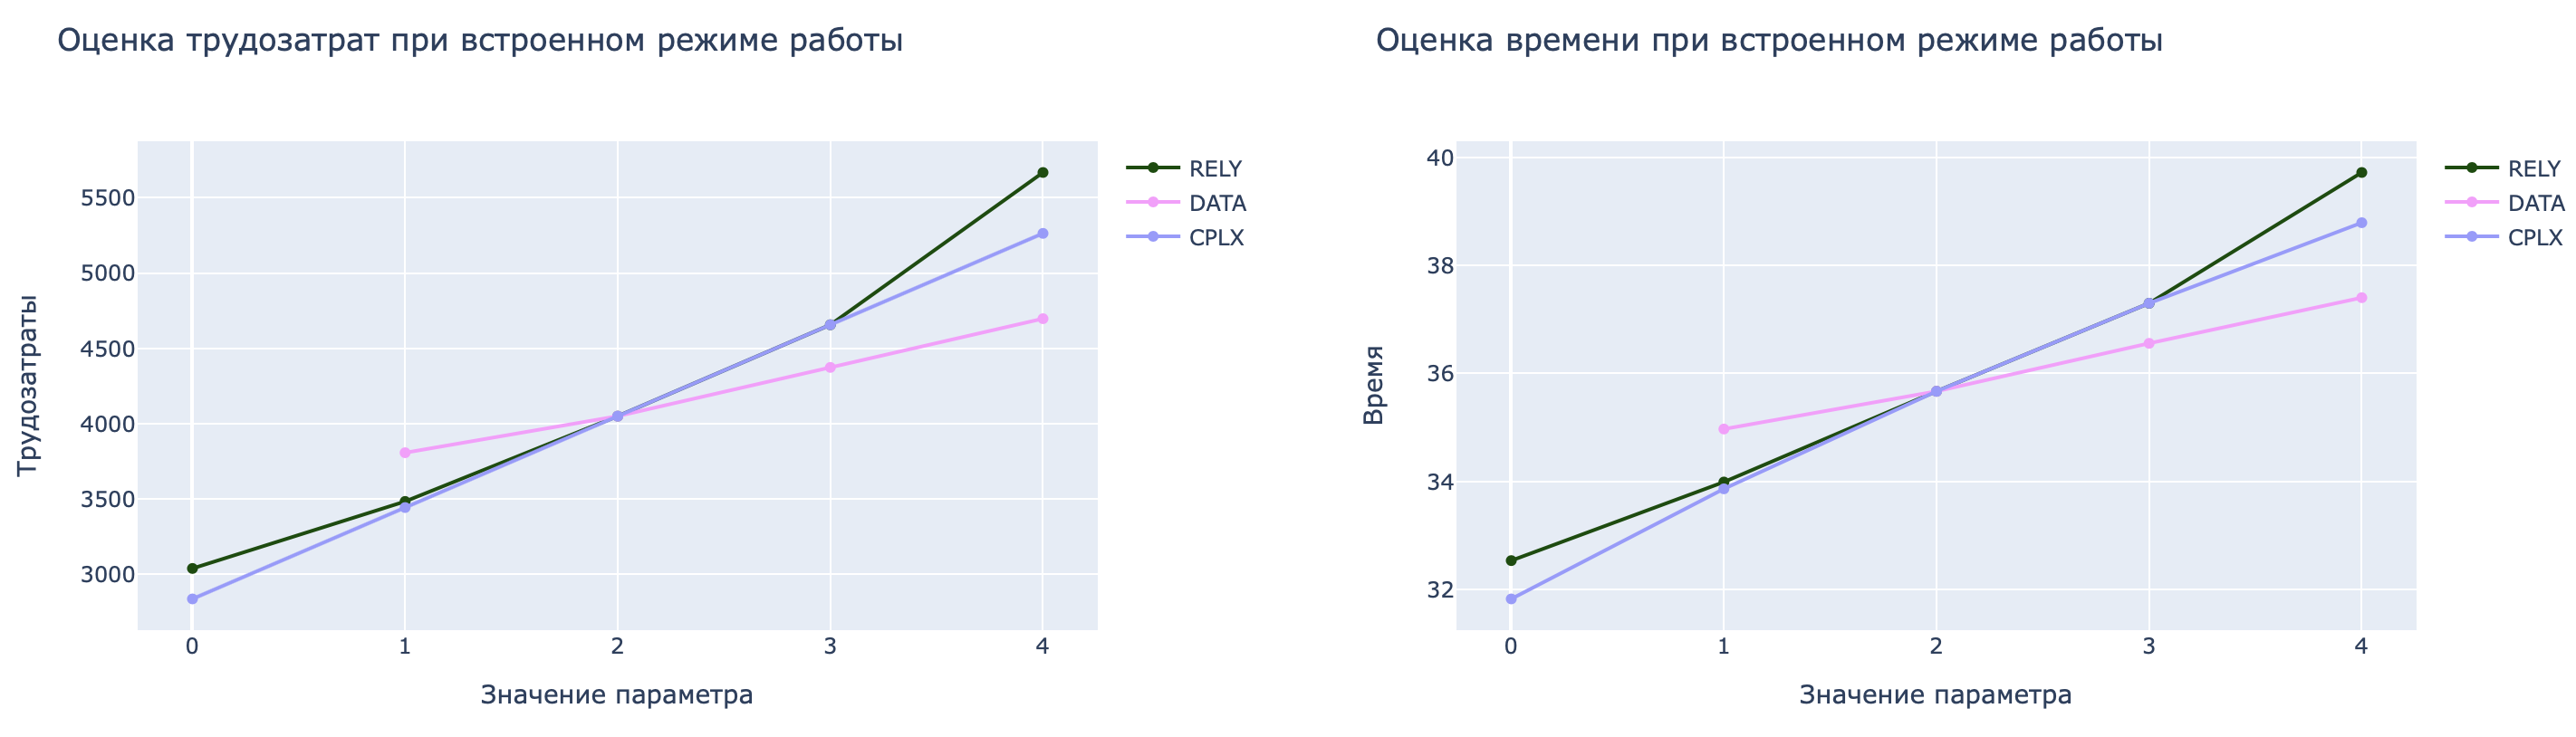
\includegraphics[scale=0.4]{bltin}
\end{figure}

Как видно из графиков выше, от изменения уровня факторов, меняет значения трудозатрат и времени -- повышаются.

Наибольшее влияние оказывает уровень фактора RELY, он потребует самую долгое время разработки и трудозатрат. Но при уровне DATA = низкий, его влияние оказывается больше.

Теперь добавим более жесткое ограничение на время выполнения.

\begin{figure}[H]
  \centering
  \caption{Изменение атрибута времени. }
  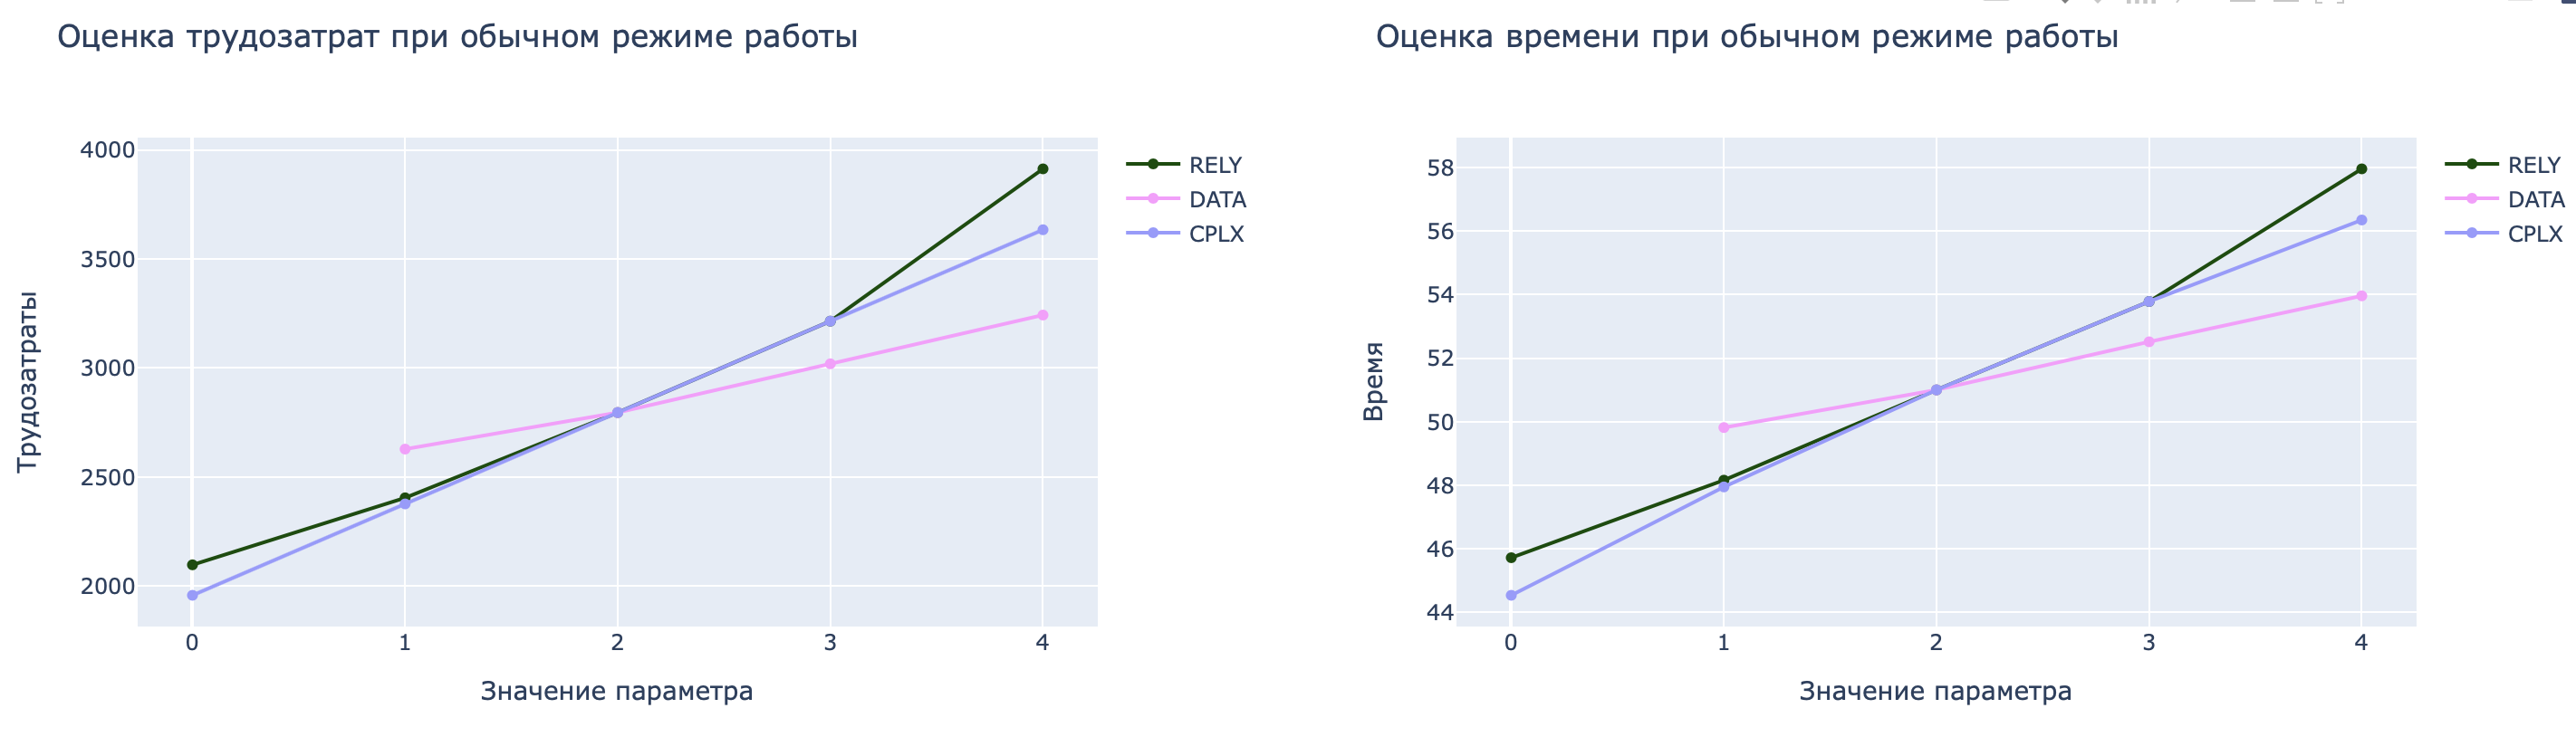
\includegraphics[scale=0.4]{time}
\end{figure}

При ограничении времени выполнения увеличатся трудозатраты и время разработки. 

\item \textbf{Рассчитать показатели проекта.}

Компания разрабатывает программную систему управления воздушным движением. Программа обрабатывает сигналы радара и ответчика и преобразовывает их в цифровые данные, позволяющие авиадиспетчерам назначать курсы, высоту и скорость полетов. Разработка ведется командой высококвалифицированных специалистов в рамках государственного контракта. Предполагаемый размер разрабатываемой системы 430 000 строк кода. Система имеет высокие требования по надежности, жесткие ограничения на время выполнения и сроки разработки. Используется промежуточный режим модели.

По описанию проекта, были выбраны следующие уровни факторов:

RELY = Высокий

TIME = Очень высокий

SCED = Очень высокий

Все атрибуты персонала высокие.

CPLX = Высокий

\begin{figure}[H]
  \centering
  \caption{Атрибуты. }
  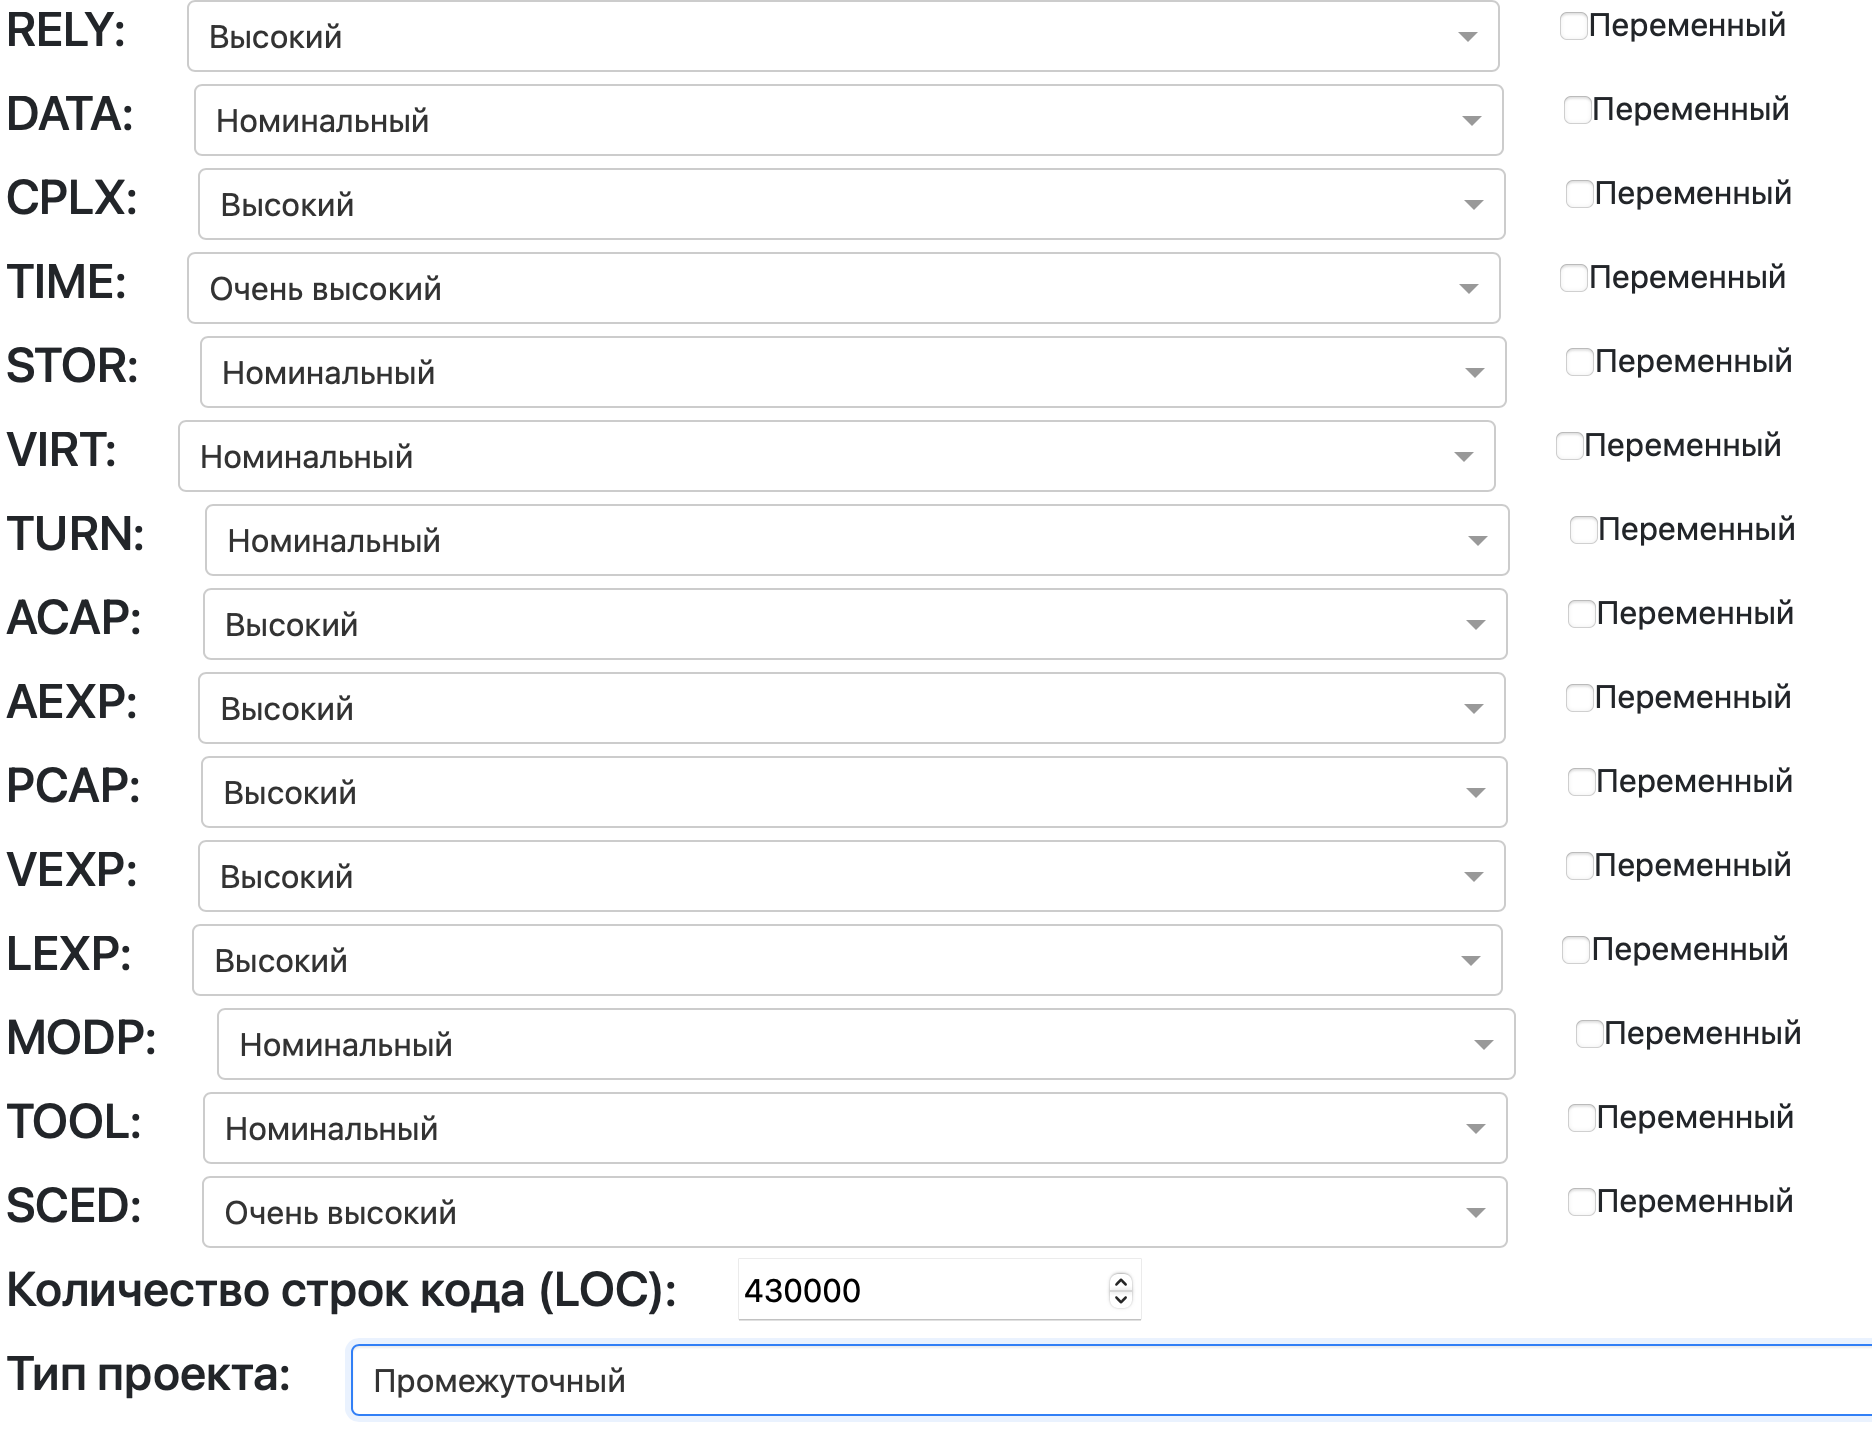
\includegraphics[scale=0.5]{table2}
\end{figure}

Тогда

\begin{figure}[H]
  \centering
  \caption{Трудозатраты, время и распределение работ. }
  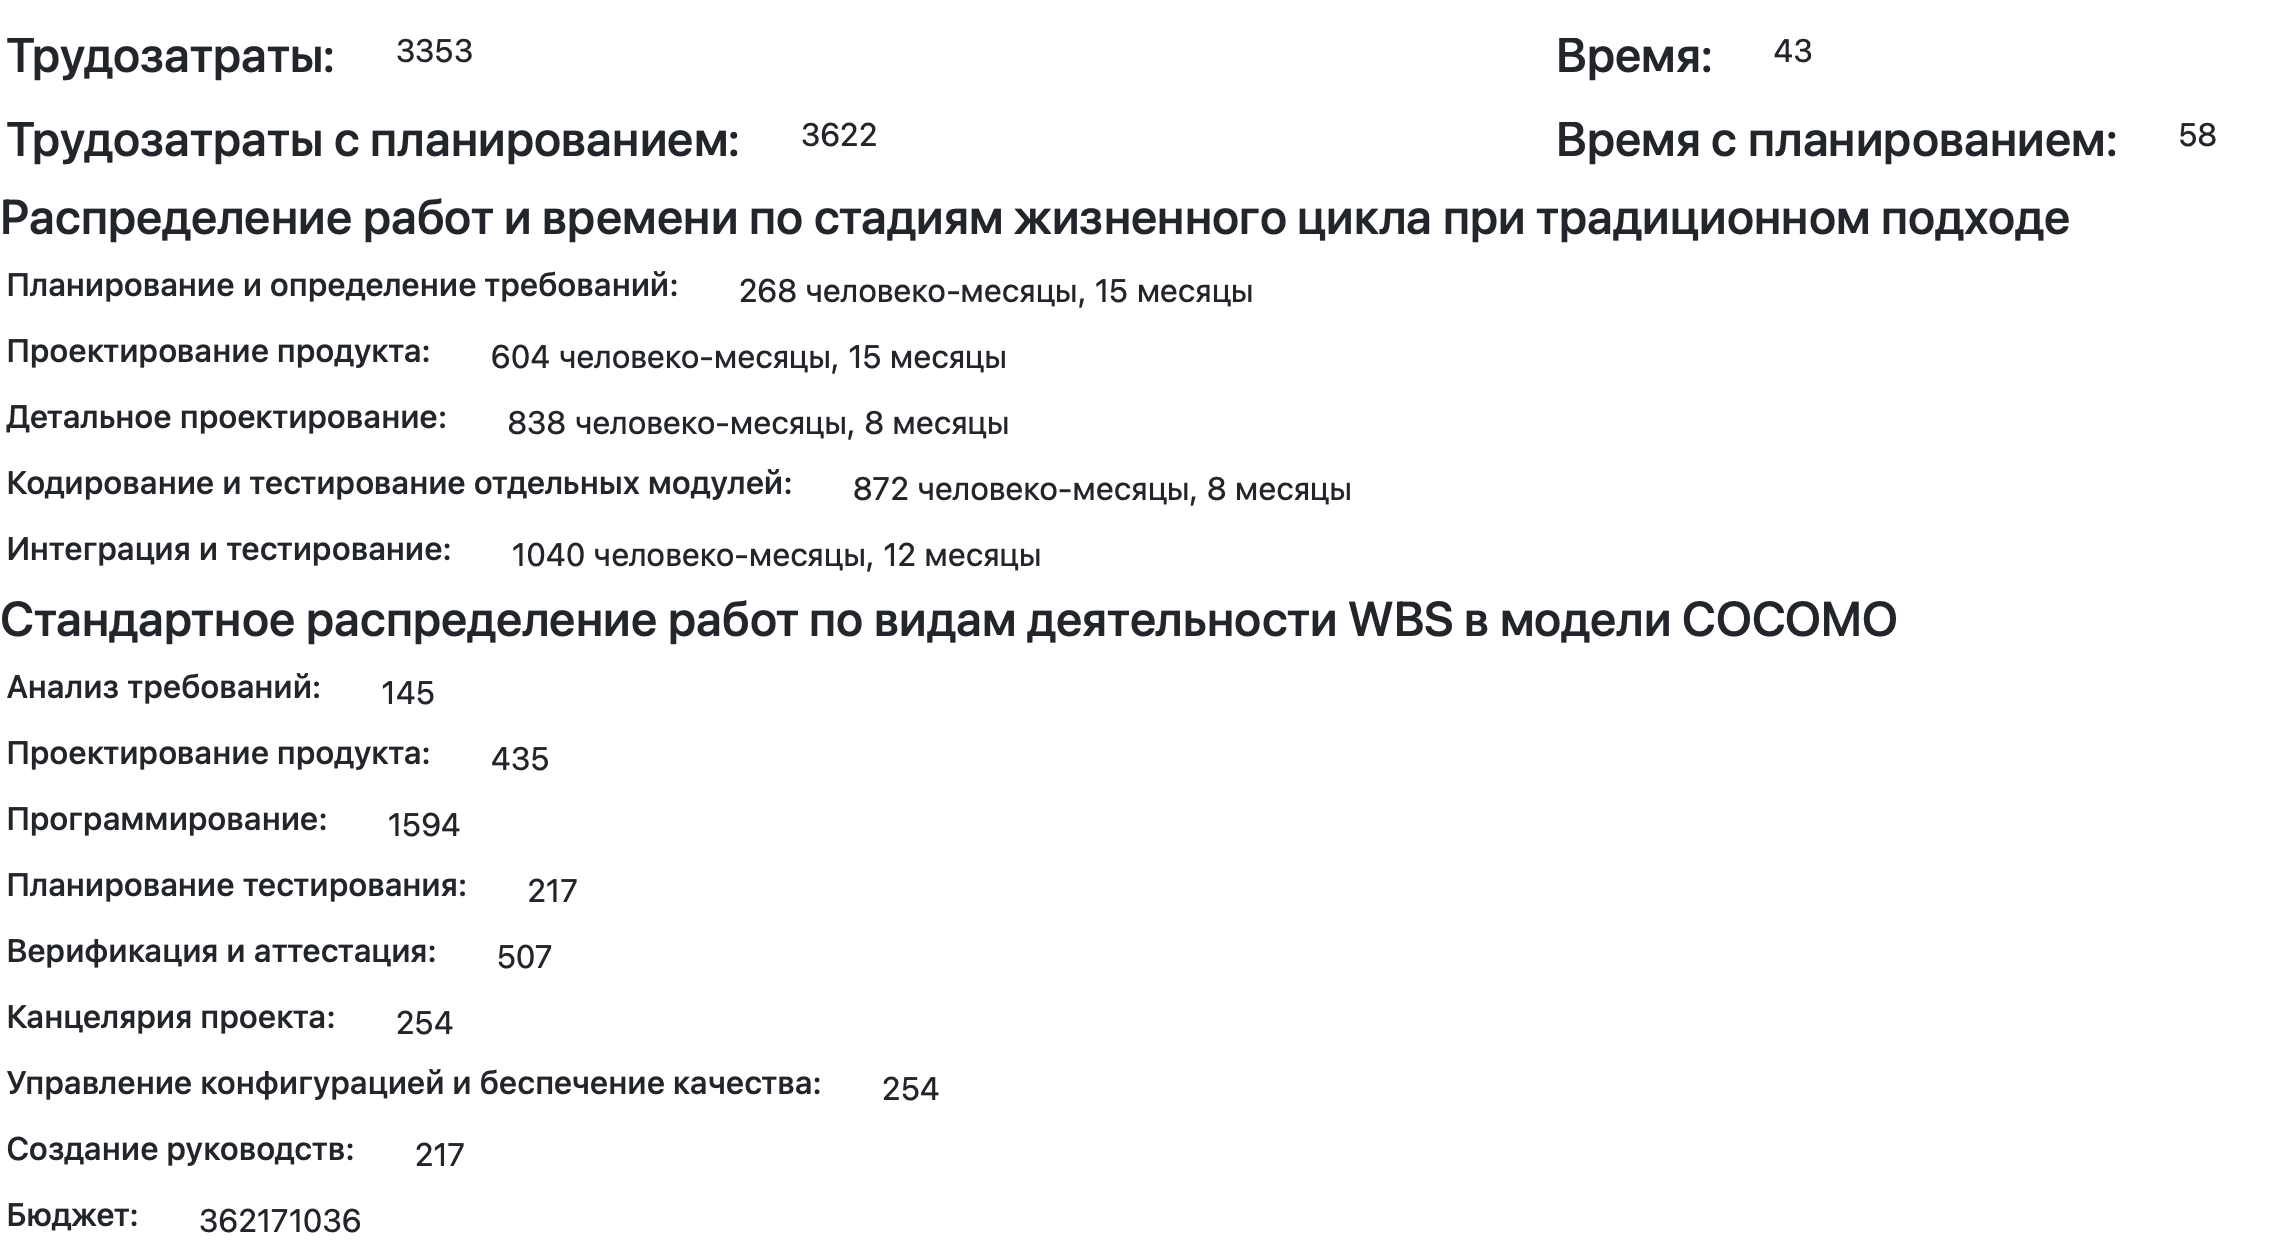
\includegraphics[scale=0.4]{project}
\end{figure}

\begin{figure}[H]
  \centering
  \caption{Количество работников. }
  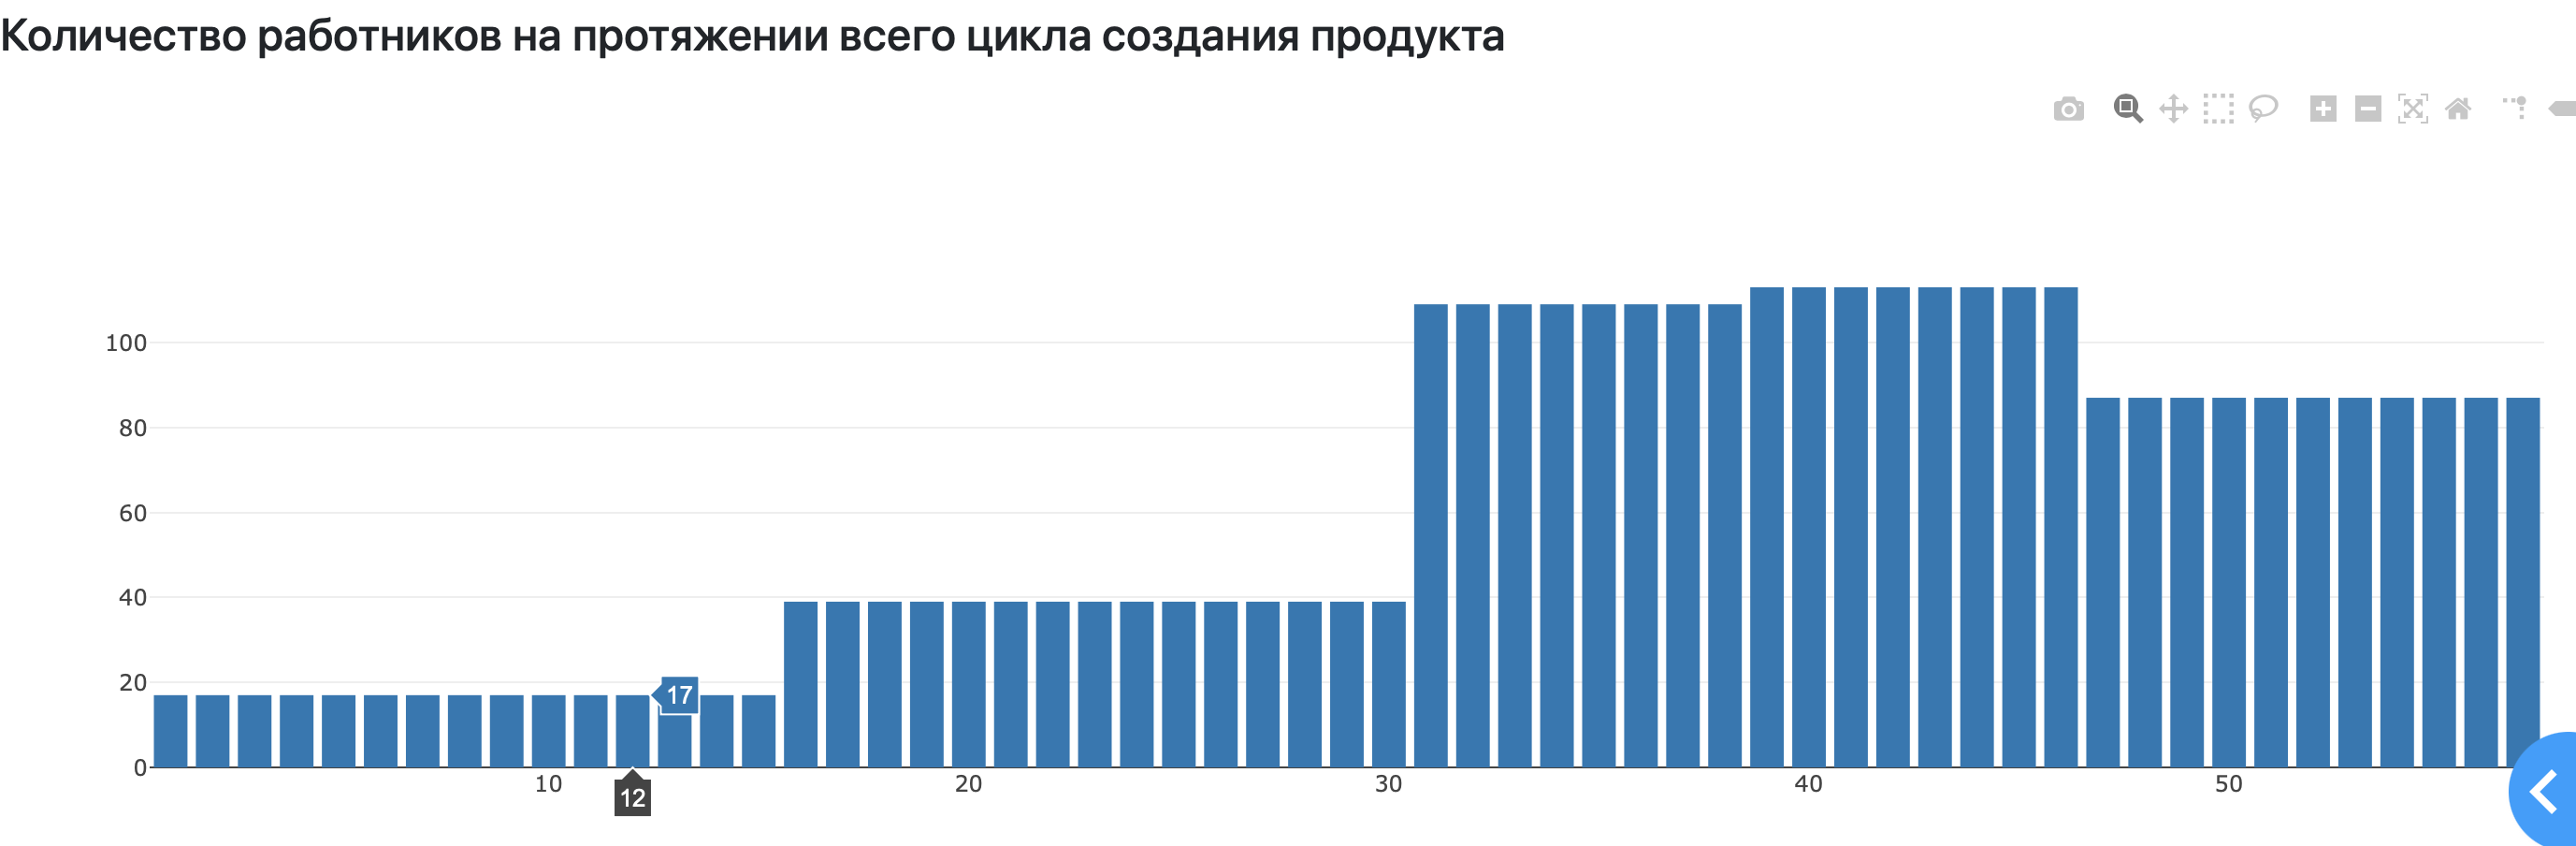
\includegraphics[scale=0.4]{count}
\end{figure}

\item \textbf{Вывод.}

Использование метода COCOMO позволяет дать первичную оценку проекта, используя только знания о количестве строк кода(LOC) и параметрах проекта. 

Но стоит учитывать, что уже существует COCOMO 2, которая может учесть также человеческие факторы: например сплоченность команды или влияние заказчика, а также по отдельности оценивать различные составляющие проекта. 

\end{enumerate}

\end{document}